

\tikzset{every picture/.style={line width=0.75pt}} %set default line width to 0.75pt        

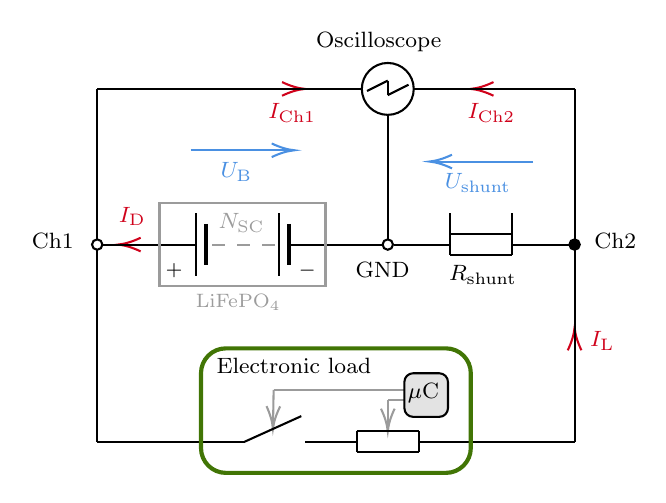
\begin{tikzpicture}[x=0.75pt,y=0.75pt,yscale=-1,xscale=1]
%uncomment if require: \path (0,743); %set diagram left start at 0, and has height of 743

%Straight Lines [id:da045931729156849066] 
\draw [color={rgb, 255:red, 208; green, 2; blue, 27 }  ,draw opacity=1 ]   (285,105) -- (272,105) ;
\draw [shift={(270,105)}, rotate = 360] [color={rgb, 255:red, 208; green, 2; blue, 27 }  ,draw opacity=1 ][line width=0.75]    (10.93,-3.29) .. controls (6.95,-1.4) and (3.31,-0.3) .. (0,0) .. controls (3.31,0.3) and (6.95,1.4) .. (10.93,3.29)   ;
%Straight Lines [id:da3949134308814568] 
\draw    (270,275) -- (320,275) ;
%Straight Lines [id:da08560996153222833] 
\draw [color={rgb, 255:red, 208; green, 2; blue, 27 }  ,draw opacity=1 ]   (115,180) -- (102,180) ;
\draw [shift={(100,180)}, rotate = 360] [color={rgb, 255:red, 208; green, 2; blue, 27 }  ,draw opacity=1 ][line width=0.75]    (10.93,-3.29) .. controls (6.95,-1.4) and (3.31,-0.3) .. (0,0) .. controls (3.31,0.3) and (6.95,1.4) .. (10.93,3.29)   ;
%Straight Lines [id:da050616828595225094] 
\draw    (92.5,180) -- (120.5,180) ;
%Straight Lines [id:da6370801814614784] 
\draw    (200.5,180) -- (227.5,180) ;
%Straight Lines [id:da4527627205165792] 
\draw [color={rgb, 255:red, 208; green, 2; blue, 27 }  ,draw opacity=1 ]   (320,235) -- (320,222) ;
\draw [shift={(320,220)}, rotate = 450] [color={rgb, 255:red, 208; green, 2; blue, 27 }  ,draw opacity=1 ][line width=0.75]    (10.93,-3.29) .. controls (6.95,-1.4) and (3.31,-0.3) .. (0,0) .. controls (3.31,0.3) and (6.95,1.4) .. (10.93,3.29)   ;
%Straight Lines [id:da4189378099752894] 
\draw [color={rgb, 255:red, 208; green, 2; blue, 27 }  ,draw opacity=1 ]   (175,105) -- (188,105) ;
\draw [shift={(190,105)}, rotate = 180] [color={rgb, 255:red, 208; green, 2; blue, 27 }  ,draw opacity=1 ][line width=0.75]    (10.93,-3.29) .. controls (6.95,-1.4) and (3.31,-0.3) .. (0,0) .. controls (3.31,0.3) and (6.95,1.4) .. (10.93,3.29)   ;
%Straight Lines [id:da2658092860751087] 
\draw [line width=0.75]    (137.5,165) -- (137.5,195) ;
%Straight Lines [id:da3949939895399093] 
\draw [color={rgb, 255:red, 155; green, 155; blue, 155 }  ,draw opacity=1 ] [dash pattern={on 4.5pt off 4.5pt}]  (175.5,180) -- (140.5,180) ;
%Straight Lines [id:da6668323928749316] 
\draw [line width=1.5]    (142.5,170) -- (142.5,190) ;
%Straight Lines [id:da2892580654722863] 
\draw [line width=0.75]    (177.5,165) -- (177.5,195) ;
%Straight Lines [id:da305974803365608] 
\draw [line width=1.5]    (182.5,170) -- (182.5,190) ;
%Straight Lines [id:da02397573109880402] 
\draw    (137.5,180) -- (120.5,180) ;
%Straight Lines [id:da31190085768960363] 
\draw    (199.5,180) -- (182.5,180) ;
%Shape: Rectangle [id:dp8008725070360889] 
\draw  [color={rgb, 255:red, 155; green, 155; blue, 155 }  ,draw opacity=1 ] (200,160) -- (200,200) -- (120,200) -- (120,160) -- cycle ;
%Shape: Circle [id:dp20223673484144356] 
\draw   (227.5,180) .. controls (227.5,178.62) and (228.62,177.5) .. (230,177.5) .. controls (231.38,177.5) and (232.5,178.62) .. (232.5,180) .. controls (232.5,181.38) and (231.38,182.5) .. (230,182.5) .. controls (228.62,182.5) and (227.5,181.38) .. (227.5,180) -- cycle ;
%Shape: Circle [id:dp3853206170680481] 
\draw   (87.5,180) .. controls (87.5,178.62) and (88.62,177.5) .. (90,177.5) .. controls (91.38,177.5) and (92.5,178.62) .. (92.5,180) .. controls (92.5,181.38) and (91.38,182.5) .. (90,182.5) .. controls (88.62,182.5) and (87.5,181.38) .. (87.5,180) -- cycle ;
%Straight Lines [id:da5327428480980583] 
\draw    (90,105) -- (90,177.5) ;
%Straight Lines [id:da13935190161788125] 
\draw    (90,105) -- (217.5,105) ;
%Straight Lines [id:da7865577264880768] 
\draw [color={rgb, 255:red, 74; green, 144; blue, 226 }  ,draw opacity=1 ]   (135,134.57) -- (183,134.57) ;
\draw [shift={(185,134.57)}, rotate = 180] [color={rgb, 255:red, 74; green, 144; blue, 226 }  ,draw opacity=1 ][line width=0.75]    (10.93,-3.29) .. controls (6.95,-1.4) and (3.31,-0.3) .. (0,0) .. controls (3.31,0.3) and (6.95,1.4) .. (10.93,3.29)   ;
%Shape: Circle [id:dp3317910125615249] 
\draw   (217.5,105) .. controls (217.5,98.1) and (223.1,92.5) .. (230,92.5) .. controls (236.9,92.5) and (242.5,98.1) .. (242.5,105) .. controls (242.5,111.9) and (236.9,117.5) .. (230,117.5) .. controls (223.1,117.5) and (217.5,111.9) .. (217.5,105) -- cycle ;
%Straight Lines [id:da1875474942123041] 
\draw    (220,106) -- (230,101) ;
%Straight Lines [id:da4090541258718201] 
\draw    (230,101) -- (230,108) ;
%Straight Lines [id:da7457893967384179] 
\draw    (230,108) -- (240,103) ;

%Straight Lines [id:da0917057683123701] 
\draw    (90,182.5) -- (90,275) ;
%Straight Lines [id:da2778004994432466] 
\draw [color={rgb, 255:red, 155; green, 155; blue, 155 }  ,draw opacity=1 ]   (230,255) -- (230,268) ;
\draw [shift={(230,270)}, rotate = 270] [color={rgb, 255:red, 155; green, 155; blue, 155 }  ,draw opacity=1 ][line width=0.75]    (10.93,-3.29) .. controls (6.95,-1.4) and (3.31,-0.3) .. (0,0) .. controls (3.31,0.3) and (6.95,1.4) .. (10.93,3.29)   ;
%Straight Lines [id:da32924484737520543] 
\draw    (245,280) -- (245,270) ;
%Straight Lines [id:da33462944952545204] 
\draw    (215,280) -- (215,270) ;
%Straight Lines [id:da24868968049308626] 
\draw    (215,270) -- (245,270) ;
%Straight Lines [id:da6617574409624216] 
\draw    (215,280) -- (245,280) ;
%Straight Lines [id:da8690193038101492] 
\draw    (215,275) -- (200,275) ;
%Straight Lines [id:da7998432795618544] 
\draw [color={rgb, 255:red, 155; green, 155; blue, 155 }  ,draw opacity=1 ]   (238,255) -- (230,255) ;
%Straight Lines [id:da10758294037064475] 
\draw    (270,275) -- (245,275) ;
%Straight Lines [id:da6790087801319198] 
\draw    (90,275) -- (140,275) ;
%Straight Lines [id:da7635403190384071] 
\draw [color={rgb, 255:red, 155; green, 155; blue, 155 }  ,draw opacity=1 ]   (174.71,266.83) -- (175,250) ;
\draw [shift={(174.67,268.83)}, rotate = 271] [color={rgb, 255:red, 155; green, 155; blue, 155 }  ,draw opacity=1 ][line width=0.75]    (10.93,-3.29) .. controls (6.95,-1.4) and (3.31,-0.3) .. (0,0) .. controls (3.31,0.3) and (6.95,1.4) .. (10.93,3.29)   ;
%Straight Lines [id:da09729743826270276] 
\draw    (205,275) -- (190,275) ;
%Straight Lines [id:da1421569585710698] 
\draw    (188.34,262.65) -- (161,275) ;
%Straight Lines [id:da5452375072503128] 
\draw    (161,275) -- (140,275) ;
%Straight Lines [id:da5345291081584591] 
\draw [color={rgb, 255:red, 155; green, 155; blue, 155 }  ,draw opacity=1 ]   (238,250) -- (175,250) ;
%Rounded Rect [id:dp6576837931168715] 
\draw  [fill={rgb, 255:red, 227; green, 227; blue, 227 }  ,fill opacity=1 ] (238,246.2) .. controls (238,243.88) and (239.88,242) .. (242.2,242) -- (254.8,242) .. controls (257.12,242) and (259,243.88) .. (259,246.2) -- (259,258.8) .. controls (259,261.12) and (257.12,263) .. (254.8,263) -- (242.2,263) .. controls (239.88,263) and (238,261.12) .. (238,258.8) -- cycle ;

%Rounded Rect [id:dp11415612065842651] 
\draw  [color={rgb, 255:red, 65; green, 117; blue, 5 }  ,draw opacity=1 ][line width=1.5]  (140,242) .. controls (140,235.37) and (145.37,230) .. (152,230) -- (258,230) .. controls (264.63,230) and (270,235.37) .. (270,242) -- (270,278) .. controls (270,284.63) and (264.63,290) .. (258,290) -- (152,290) .. controls (145.37,290) and (140,284.63) .. (140,278) -- cycle ;
%Straight Lines [id:da6054782174044755] 
\draw    (320,180) -- (320,275) ;
%Straight Lines [id:da5423361466871042] 
\draw    (242.5,105) -- (320,105) ;
%Straight Lines [id:da9479324460356069] 
\draw    (290,185) -- (290,175) ;
%Straight Lines [id:da8225786744388688] 
\draw    (260,185) -- (260,175) ;
%Straight Lines [id:da05714096809956737] 
\draw    (260,185) -- (290,185) ;
%Straight Lines [id:da8511132029064918] 
\draw    (260,175) -- (290,175) ;
%Straight Lines [id:da6701815168749929] 
\draw    (260,165) -- (260,175) ;
%Straight Lines [id:da41839660929781086] 
\draw    (290,165) -- (290,175) ;
%Shape: Circle [id:dp2800781557119969] 
\draw  [fill={rgb, 255:red, 0; green, 0; blue, 0 }  ,fill opacity=1 ] (320,177.5) .. controls (321.38,177.5) and (322.5,178.62) .. (322.5,180) .. controls (322.5,181.38) and (321.38,182.5) .. (320,182.5) .. controls (318.62,182.5) and (317.5,181.38) .. (317.5,180) .. controls (317.5,178.62) and (318.62,177.5) .. (320,177.5) -- cycle ;
%Straight Lines [id:da2549570467676723] 
\draw    (290,180) -- (320,180) ;
%Straight Lines [id:da2939345663201236] 
\draw    (233,180) -- (260,180) ;
%Straight Lines [id:da832541761407757] 
\draw    (230,117.5) -- (230,177.5) ;
%Straight Lines [id:da19404732115287238] 
\draw [color={rgb, 255:red, 74; green, 144; blue, 226 }  ,draw opacity=1 ]   (300,140) -- (252,140) ;
\draw [shift={(250,140)}, rotate = 360] [color={rgb, 255:red, 74; green, 144; blue, 226 }  ,draw opacity=1 ][line width=0.75]    (10.93,-3.29) .. controls (6.95,-1.4) and (3.31,-0.3) .. (0,0) .. controls (3.31,0.3) and (6.95,1.4) .. (10.93,3.29)   ;

%Straight Lines [id:da8406967180739828] 
\draw    (320,105) -- (320,177.5) ;

% Text Node
\draw (136,202.4) node [anchor=north west][inner sep=0.75pt]  [font=\scriptsize,color={rgb, 255:red, 0; green, 0; blue, 0 }  ,opacity=1 ]  {$\mathrm{\textcolor[rgb]{0.61,0.61,0.61}{LiFePO}\textcolor[rgb]{0.61,0.61,0.61}{_{4}}}$};
% Text Node
\draw (185.5,187.4) node [anchor=north west][inner sep=0.75pt]  [font=\scriptsize]  {$-$};
% Text Node
\draw (121.5,187.4) node [anchor=north west][inner sep=0.75pt]  [font=\scriptsize]  {$+$};
% Text Node
\draw (147,163.4) node [anchor=north west][inner sep=0.75pt]  [font=\footnotesize,color={rgb, 255:red, 155; green, 155; blue, 155 }  ,opacity=1 ]  {$N_{\mathrm{SC}}$};
% Text Node
\draw (148,138.97) node [anchor=north west][inner sep=0.75pt]  [font=\footnotesize,color={rgb, 255:red, 74; green, 144; blue, 226 }  ,opacity=1 ]  {$U_{\mathrm{B}}$};
% Text Node
\draw (99,160.4) node [anchor=north west][inner sep=0.75pt]  [font=\footnotesize,color={rgb, 255:red, 208; green, 2; blue, 27 }  ,opacity=1 ]  {$I_{\mathrm{D}}$};
% Text Node
\draw (171,110.4) node [anchor=north west][inner sep=0.75pt]  [font=\footnotesize,color={rgb, 255:red, 208; green, 2; blue, 27 }  ,opacity=1 ]  {$I_{\mathrm{Ch} 1}$};
% Text Node
\draw (194,76) node [anchor=north west][inner sep=0.75pt]  [font=\footnotesize] [align=left] {Oscilloscope};
% Text Node
\draw (146,233) node [anchor=north west][inner sep=0.75pt]  [font=\footnotesize] [align=left] {Electronic load};
% Text Node
\draw (238.2,245.4) node [anchor=north west][inner sep=0.75pt]  [font=\footnotesize]  {$\mu \mathrm{C}$};
% Text Node
\draw (326,220.4) node [anchor=north west][inner sep=0.75pt]  [font=\footnotesize,color={rgb, 255:red, 208; green, 2; blue, 27 }  ,opacity=1 ]  {$I_{\mathrm{L}}$};
% Text Node
\draw (258,188.4) node [anchor=north west][inner sep=0.75pt]  [font=\footnotesize]  {$R_{\mathrm{shunt}}$};
% Text Node
\draw (267,110.4) node [anchor=north west][inner sep=0.75pt]  [font=\footnotesize,color={rgb, 255:red, 208; green, 2; blue, 27 }  ,opacity=1 ]  {$I_{\mathrm{Ch} 2}$};
% Text Node
\draw (213,187) node [anchor=north west][inner sep=0.75pt]  [font=\footnotesize] [align=left] {GND};
% Text Node
\draw (328,173) node [anchor=north west][inner sep=0.75pt]  [font=\footnotesize] [align=left] {Ch2};
% Text Node
\draw (57,173) node [anchor=north west][inner sep=0.75pt]  [font=\footnotesize] [align=left] {Ch1};
% Text Node
\draw (256,144.4) node [anchor=north west][inner sep=0.75pt]  [font=\footnotesize,color={rgb, 255:red, 74; green, 144; blue, 226 }  ,opacity=1 ]  {$U_{\mathrm{shunt}}$};


\end{tikzpicture}
